% Title: gl2ps_renderer figure
% Creator: GL2PS 1.4.0, (C) 1999-2017 C. Geuzaine
% For: Octave
% CreationDate: Sun Dec  1 20:36:24 2019
\setlength{\unitlength}{1pt}
\begin{picture}(0,0)
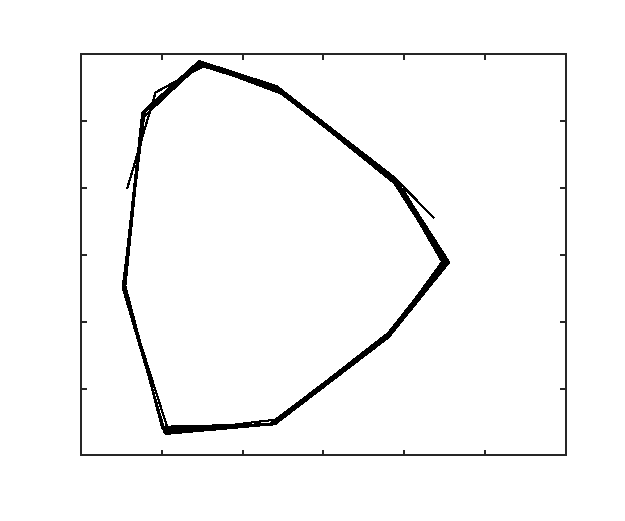
\includegraphics{img/phaseThetaPTheta-inc}
\end{picture}%
\begin{picture}(300,250)(0,0)
\fontsize{10}{0}
\selectfont\put(39,24){\makebox(0,0)[t]{\textcolor[rgb]{0.15,0.15,0.15}{{0.2}}}}
\fontsize{10}{0}
\selectfont\put(77.75,24){\makebox(0,0)[t]{\textcolor[rgb]{0.15,0.15,0.15}{{0.4}}}}
\fontsize{10}{0}
\selectfont\put(116.5,24){\makebox(0,0)[t]{\textcolor[rgb]{0.15,0.15,0.15}{{0.6}}}}
\fontsize{10}{0}
\selectfont\put(155.25,24){\makebox(0,0)[t]{\textcolor[rgb]{0.15,0.15,0.15}{{0.8}}}}
\fontsize{10}{0}
\selectfont\put(194,24){\makebox(0,0)[t]{\textcolor[rgb]{0.15,0.15,0.15}{{1}}}}
\fontsize{10}{0}
\selectfont\put(232.75,24){\makebox(0,0)[t]{\textcolor[rgb]{0.15,0.15,0.15}{{1.2}}}}
\fontsize{10}{0}
\selectfont\put(271.5,24){\makebox(0,0)[t]{\textcolor[rgb]{0.15,0.15,0.15}{{1.4}}}}
\fontsize{10}{0}
\selectfont\put(34.0107,31.4813){\makebox(0,0)[r]{\textcolor[rgb]{0.15,0.15,0.15}{{-3}}}}
\fontsize{10}{0}
\selectfont\put(34.0107,63.5677){\makebox(0,0)[r]{\textcolor[rgb]{0.15,0.15,0.15}{{-2}}}}
\fontsize{10}{0}
\selectfont\put(34.0107,95.6542){\makebox(0,0)[r]{\textcolor[rgb]{0.15,0.15,0.15}{{-1}}}}
\fontsize{10}{0}
\selectfont\put(34.0107,127.741){\makebox(0,0)[r]{\textcolor[rgb]{0.15,0.15,0.15}{{0}}}}
\fontsize{10}{0}
\selectfont\put(34.0107,159.827){\makebox(0,0)[r]{\textcolor[rgb]{0.15,0.15,0.15}{{1}}}}
\fontsize{10}{0}
\selectfont\put(34.0107,191.914){\makebox(0,0)[r]{\textcolor[rgb]{0.15,0.15,0.15}{{2}}}}
\fontsize{10}{0}
\selectfont\put(34.0107,224){\makebox(0,0)[r]{\textcolor[rgb]{0.15,0.15,0.15}{{3}}}}
\fontsize{11}{0}
\selectfont\put(155.25,11){\makebox(0,0)[t]{\textcolor[rgb]{0.15,0.15,0.15}{{$\theta$}}}}
\fontsize{11}{0}
\selectfont\put(20.0107,127.741){\rotatebox{90}{\makebox(0,0)[b]{\textcolor[rgb]{0.15,0.15,0.15}{{$p_{\theta}$}}}}}
\fontsize{11}{0}
\selectfont\put(155.25,234){\makebox(0,0)[b]{\textcolor[rgb]{0,0,0}{{Diagrama fase $\theta - p_\theta$}}}}
\end{picture}
